\chapter{Experimental evaluation for a simple problem}

Before moving on to a Multi-instance target propagation problem, the target propagation method was tested on a simple problem. The dataset used as such a "toy" problem is the \VUname{two-moon dataset}.

\section{The two-moon dataset}
The dataset consists of 2D spatial data. Each datum is a point in the \( \left( 0, 1 \right) \times \left( 0, 1 \right) \) space. The data is split into two classes, each forming a distinct shape of a crescent moon when plotted (see figure \ref{twomoon}). The two moons are inter-twinned, making the dataset not linearly separable. The actual dataset used was generated as follows:

The negative class was generated by drawing \( x \sim \mathcal{U} \left( 0.3, 0.9 \right) \) and calculating
\[ y = -2 \sqrt{0.3^2 - \left( x - 0.6 \right)^2} + 0.7 \]
This means the points lie on an ellipse with the center at \( \begin{pmatrix} 0.6 \\ 0.7 \end{pmatrix} \) and a semi-major and a semi-minor axis of \( 0.3 \) and \( 0.6 \).

The positive class was generated by drawing \( x \sim \mathcal{U} \left( 0.1, 0.7 \right) \) and calculating
\[ y = 2 \sqrt{0.3^2 - \left( x - 0.4 \right)^2} + 0.3 \]
This means the points lie on an ellipse with the center at \( \begin{pmatrix} 0.4 \\ 0.3 \end{pmatrix} \) and a semi-major and a semi-minor axis of \( 0.3 \) and \( 0.6 \), the same as for the negative class.

A random noise was added to both elements of all data points in both classes. The noise was drawn from \( \mathcal{N} \left(0, 0.025 \right) \).

\begin{figure}
	\centering
	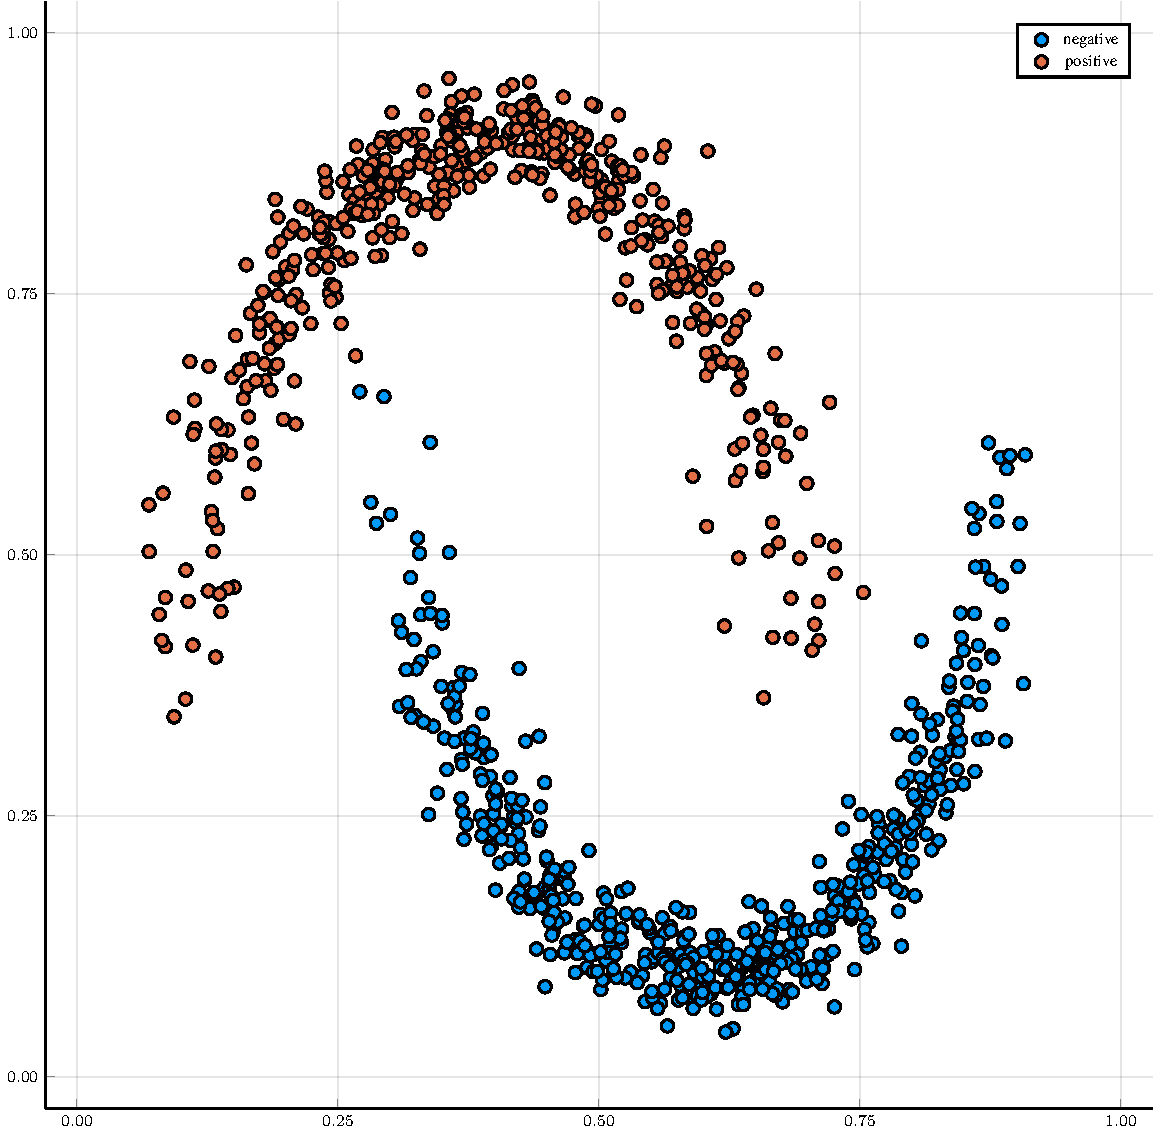
\includegraphics[width=\textwidth]{images/two-moon/two-moon.pdf}
	\caption{Example of a Two-moon dataset}\label{twomoon}
\end{figure}

\todo{Backprop on this DS}

\section{The used model}

The model used to classify these samples is a layer of 16 neurons, followed by a layer of 2 neurons, followed by the softmax function in order to represent the output as a measure of confidence that a given sample belongs to a given class. The activations used for the neurons were the tanh function, the ReLU function (see \cite{hahnloser_digital_2000}) and the swish function (see \cite{ramachandran_searching_2018}). ADAM (see \cite{kingma_adam:_2014}) was used as the optimisation method. The mean squared error function was used as the model loss as well as the layer-local loss function for all the layers. The training dataset consisted of a 1000 random samples, the testing dataset was 100 samples. The network was taught on the training dataset in 2000 epochs.

To learn the inverse mappings the same model was used for both of the first two layers. This model consisted of a layer of 8 neurons followed by a layer with as many neurons as was the required input dimension. The second of those used identity as an activation function, the first used the same activation as the rest of the network. The inverse mapping for the softmax function consisted of a layer of 4 neurons followed by a layer of 2 neurons with the identity function as its activation. The mean squared error function was used as the dual layer-local loss function for all the inverse mappings. The noise inserted for the auto-encoder training was \( \varepsilon \sim N \left( 0, 0.2 \right) \). The step size for the last layer target (see equation \ref{targetprop_last_layer_target}) was \( \eta = 0.5 \).

\section{Results}

The model was tested with 3 activation functions. For each of these activation functions, a heatmap of predictions in the whole \( \left( 0, 1 \right) \times \left( 0, 1 \right) \) space was plotted to visualise the results. Also, a record of model loss on the testing dataset was kept, although no training was ever done on the testing dataset. For the results, see figures \ref{tanh}, \ref{relu}, \ref{swish}. \todo{Scaling}

As can be seen from the figures, the model fails to learn a classifier of the two-moon dataset. \todo{compare to backprop} An explanation of this behaviour is attempted in the following sections. Because the behaviour is very similar for all three used activations, only the ReLU activation will be considered further on.

\begin{figure}
	\centering
	\begin{subfigure}{0.49\textwidth}
		\centering
		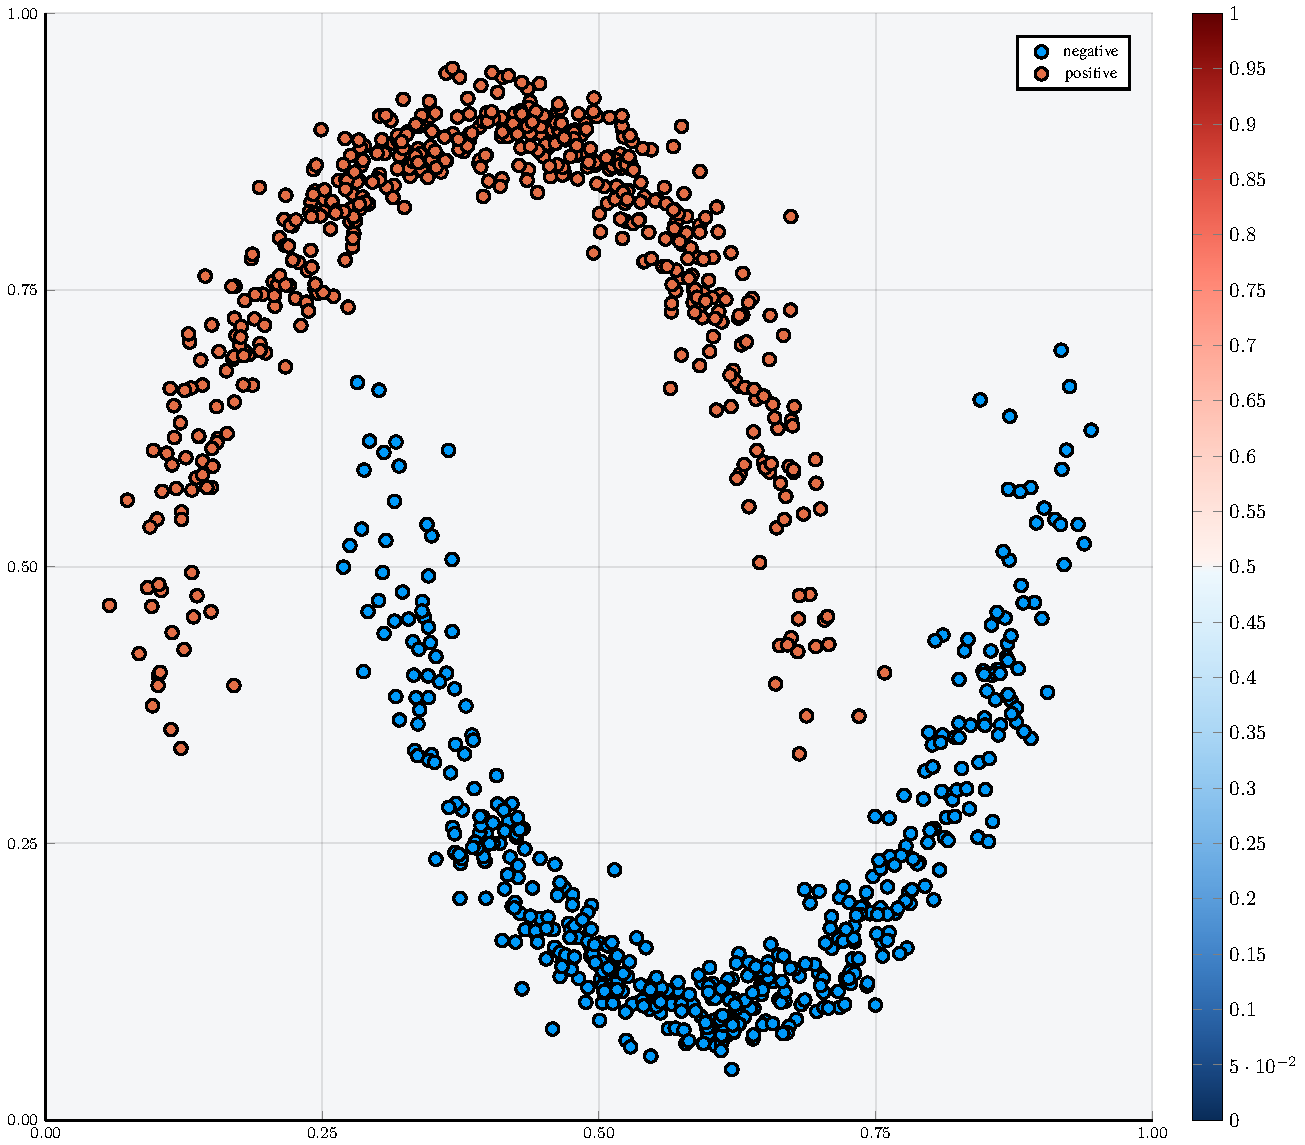
\includegraphics[width=\textwidth]{images/tanh-heatmap/tanh.pdf}
		\caption{Heatmap of model predictions on \( \left( 0, 1 \right) \times \left( 0, 1 \right) \) overlaid by the testing dataset.}
	\end{subfigure}
	\begin{subfigure}{0.49\textwidth}
		\centering
		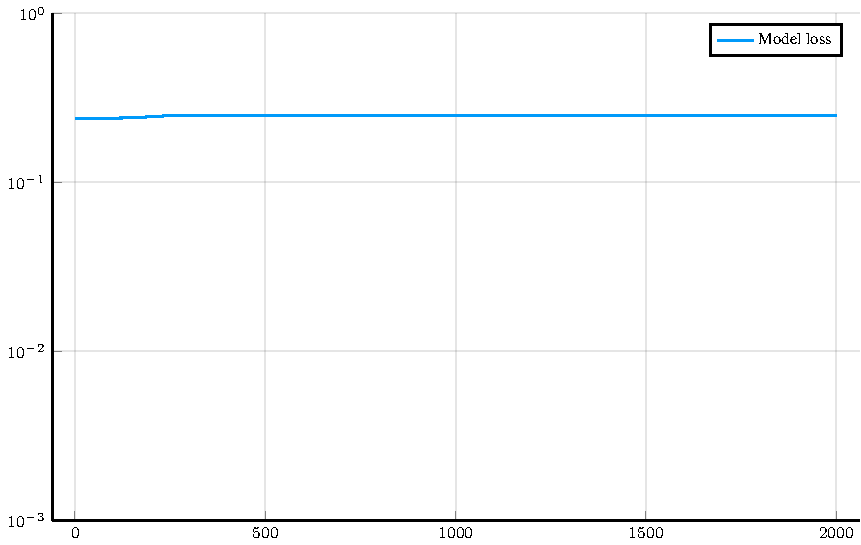
\includegraphics[width=\textwidth]{images/tanh-modelloss/tanh.pdf}
		\caption{Model loss on the testing dataset over 2000 epochs of training}
	\end{subfigure}
	\caption{Results with the tanh activation function.}\label{tanh}
\end{figure}

\begin{figure}
	\centering
	\begin{subfigure}{0.49\textwidth}
		\centering
		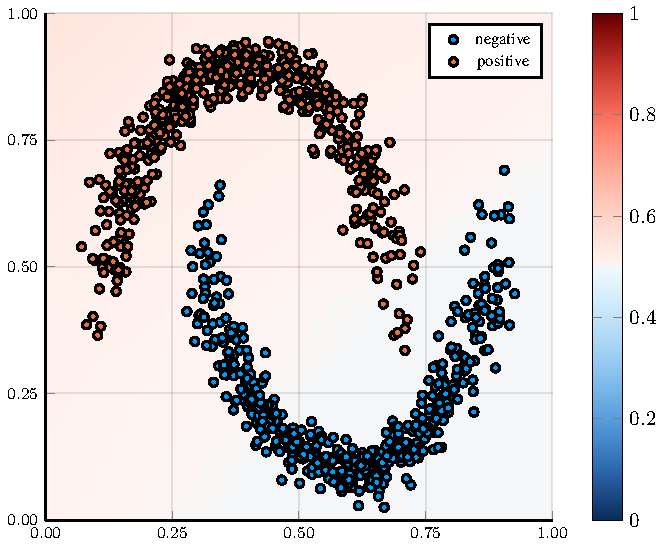
\includegraphics[width=\textwidth]{images/relu-heatmap/relu.pdf}
		\caption{Heatmap of model predictions on \( \left( 0, 1 \right) \times \left( 0, 1 \right) \) overlaid by the testing dataset.}
	\end{subfigure}
	\begin{subfigure}{0.49\textwidth}
		\centering
		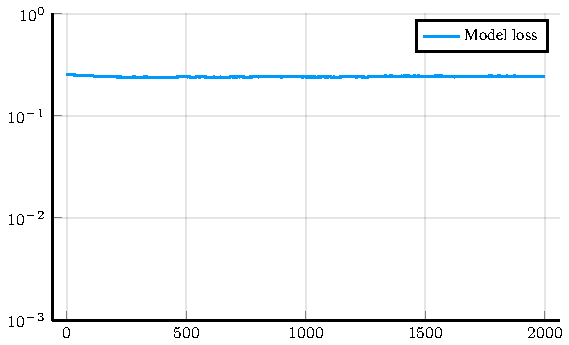
\includegraphics[width=\textwidth]{images/relu-modelloss/relu.pdf}
		\caption{Model loss on the testing dataset over 2000 epochs of training}
	\end{subfigure}
	\caption{Results with the ReLU activation function.}\label{relu}
\end{figure}

\begin{figure}
	\centering
	\begin{subfigure}{0.49\textwidth}
		\centering
		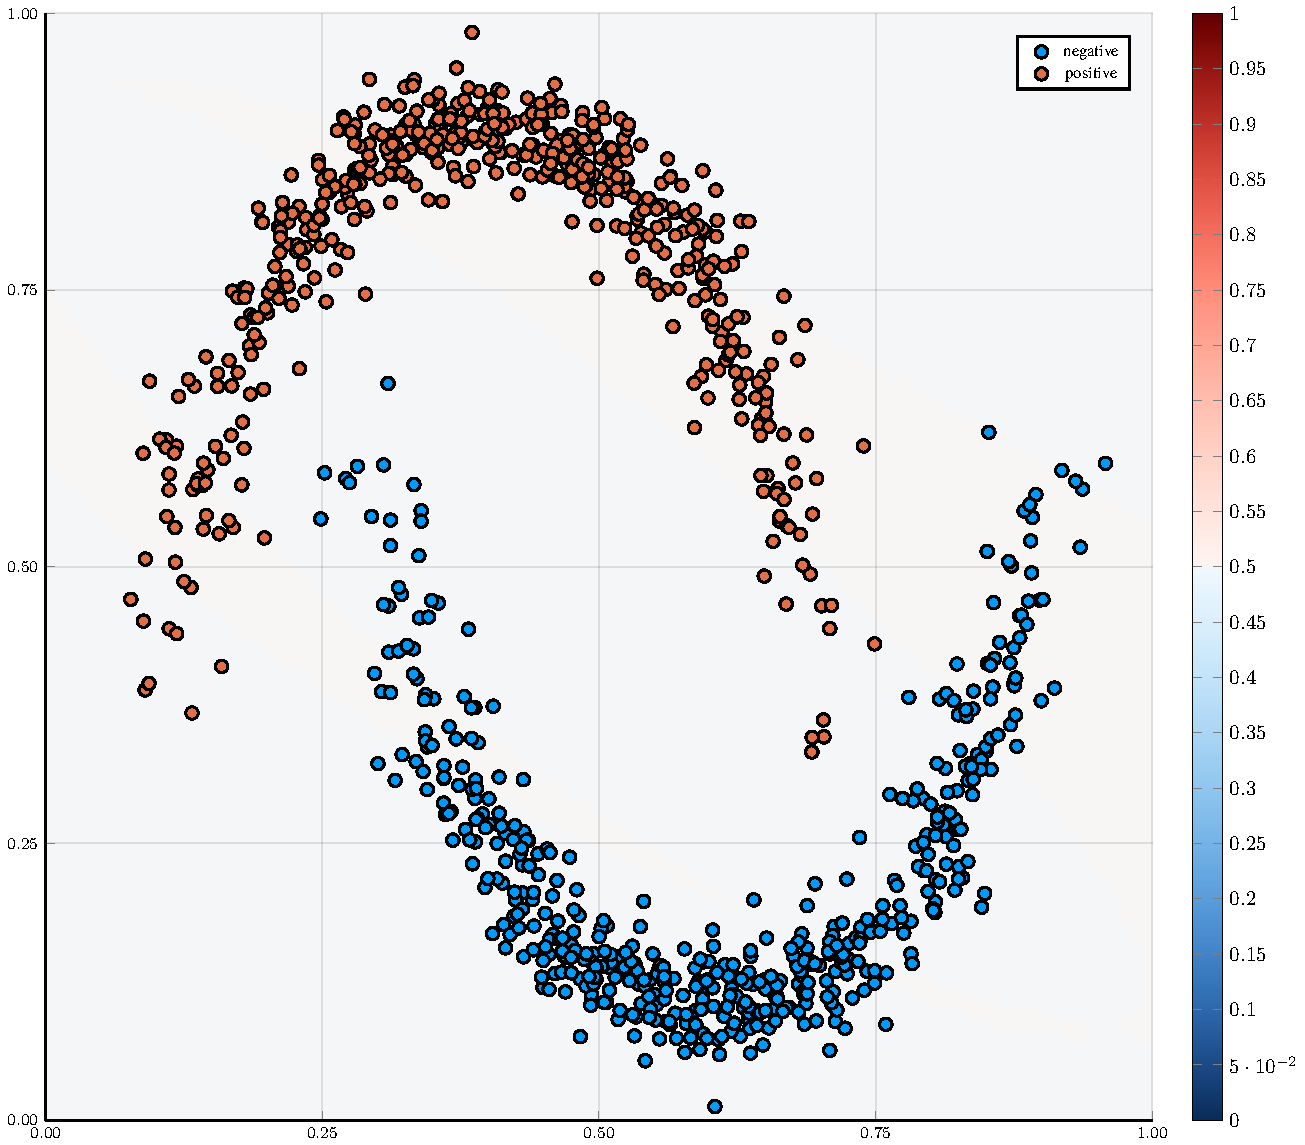
\includegraphics[width=\textwidth]{images/swish-heatmap/swish.pdf}
		\caption{Heatmap of model predictions on \( \left( 0, 1 \right) \times \left( 0, 1 \right) \) overlaid by the testing dataset.}
	\end{subfigure}
	\begin{subfigure}{0.49\textwidth}
		\centering
		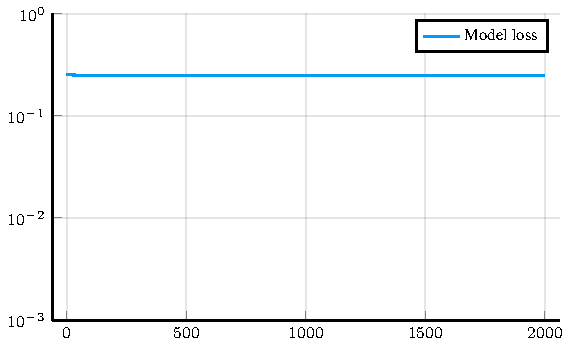
\includegraphics[width=\textwidth]{images/swish-modelloss/swish.pdf}
		\caption{Model loss on the testing dataset over 2000 epochs of training}
	\end{subfigure}
	\caption{Results with the swish activation function.}\label{swish}
\end{figure}

\section{Explanation of the results}

As a result of the architecture of a target-propagation model, the most crucial layer for the learning is the last layer, particularly the inverse mapping (i. e. the auto-encoder). The reasoning behind this claim is that if the calculated inverse function doesn't coincide with the actual inverse function, the computed target for the previous layer doesn't represent the desired target. That in turns means that the previous layer doesn't properly learn, which in turn makes its dual layer not learn the desired inverse, propagating the issue backwards through the whole model.

Figures \ref{layer1_losses} and \ref{layer2_losses} show the layer-local loss function (see section \ref{targetprop_general}) and the dual layer-local loss function (see section \ref{vanilla_targetprop}) values over the learning period. The failure to learn the last layer inverse is clearly manifested in the relatively high values of the dual layer-local loss function of the second layer.

\begin{figure}
	\centering
	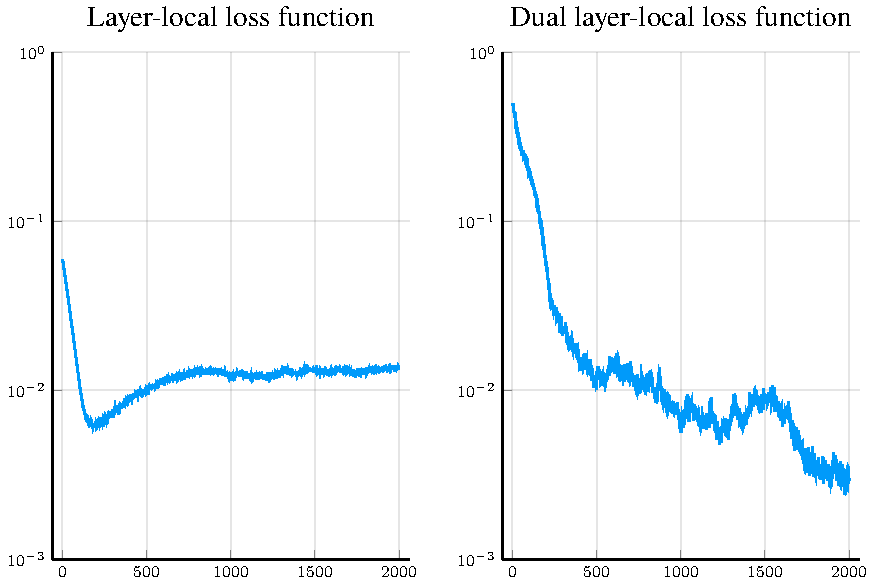
\includegraphics[width=\textwidth]{images/relu-layer1/layer1.pdf}
	\caption{Layer local losses for the first layer over 2000 epochs of training}\label{layer1_losses}
\end{figure}

\begin{figure}
	\centering
	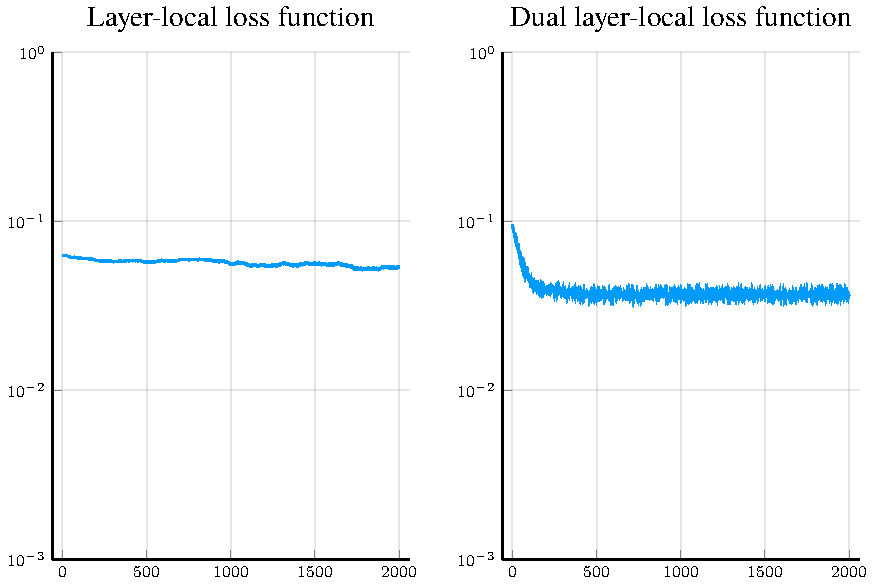
\includegraphics[width=\textwidth]{images/relu-layer2/layer2.pdf}
	\caption{Layer local losses for the second layer over 2000 epochs of training}\label{layer2_losses}
\end{figure}

\subsection{A hypothesis: The classifier is non-invertible}

A possible explanation for this phenomenon follows as such: Let \( \VUvec{x} \) be the input of the last layer, denoted \( f \). Suppose that the function \( f \) is not injective, that is there exist \( \VUvec{x}_1 \) and \( \VUvec{x}_2 \) such that \( f \left( \VUvec{x}_1 \right) = f \left( \VUvec{x}_2 \right) \). Then necessarily \( \widetilde{f}^{-1} \left( f \left( \VUvec{x}_1 \right) \right) = \widetilde{f}^{-1} \left( f \left( \VUvec{x}_2 \right) \right) \) which means that generally \( \widetilde{f}^{-1} \left( f \left( \VUvec{x} \right) \right) \not\approx \VUvec{x} \).

It is a reasonable simplification to assume the functions \( f \) and \( \widetilde{f}^{-1} \) linear due to the nature of the ReLU activation function. Under this assumption, the non-injectivity of \( f \) means that for the previously mentioned \( x_1 \) and \( x_2 \), there exist decompositions
\[ \VUvec{x}_1 = \widehat{\VUvec{x}} + \widehat{\VUvec{x}}_1^\perp \quad \text{where} \quad \widehat{\VUvec{x}}_1^\perp \in \mathrm{Ker} \left( f \right) \]
\[ \VUvec{x}_2 = \widehat{\VUvec{x}} + \widehat{\VUvec{x}}_2^\perp \quad \text{where} \quad \widehat{\VUvec{x}}_2^\perp \in \mathrm{Ker} \left( f \right) \]
Then \( f \left( \VUvec{x}_1 \right) = f \left( \VUvec{x}_2 \right) \).

\subsection{Testing the hypothesis}

A way to test test this hypothesis would be to use the property \( \VUvec{x}_1 - \VUvec{x}_2 = \VUvec{x}_1^\perp - \VUvec{x}_2^\perp \in \mathrm{Ker} \left( f \right) \). For a dataset of \( n \) samples, this would mean testing for
\begin{equation}\label{difference_test}
	f \left( \sum_{i = 1}^{n - 1} \left( \VUvec{x}_{i + 1} - \VUvec{x}_i \right) \right) = f \left( \sum_{i = 1}^{n - 1} \left( \widehat{\VUvec{x}}_{i + 1}^\perp - \widehat{\VUvec{x}}_i^\perp \right) \right) = \VUvec{0}
\end{equation}

If it is presumed that \( \widehat{\VUvec{x}}^\perp \sim \mathcal{N} \left(0, \sigma^2 \right) \), then another test may be devised using the property \( \VUvec{x}_1 + \VUvec{x}_2 = 2 \widehat{\VUvec{x}} + \widehat{\VUvec{x}}_1^\perp + \widehat{\VUvec{x}}_2^\perp \) where \( \widehat{\VUvec{x}}_1^\perp + \widehat{\VUvec{x}}_2^\perp \sim \mathcal{N} \left( 0, 2 \sigma^2 \right) \). For a dataset of \( n \) samples, this would mean that
\[ \sum_{i = 1}^n \VUvec{x}_i = n \widehat{\VUvec{x}} + \sum_{i = 1}^n \widehat{\VUvec{x}}_i^\perp \quad \text{where} \quad \sum_{i = 1}^n \widehat{\VUvec{x}}_i^\perp \sim \mathcal{N} \left( 0, n \sigma^2 \right) \]
Using the property \( X \sim \mathcal{N} \left( 0, \sigma^2 \right) \implies kX \sim \mathcal{N} \left( 0, k^2 \sigma^2 \right) \), it can be deduced that
\[ \frac{1}{n}\sum_{i = 1}^n \VUvec{x}_i = \widehat{\VUvec{x}} + \frac{1}{n}\sum_{i = 1}^n \widehat{\VUvec{x}}_i^\perp \quad \text{where} \quad \frac{1}{n}\sum_{i = 1}^n \widehat{\VUvec{x}}_i^\perp \sim \mathcal{N} \left( 0, \frac{\sigma^2}{n} \right) \]
This in turn means that
\[ \VUvec{x}_i - \frac{1}{n}\sum_{j = 1}^n \VUvec{x}_j \approx \widehat{\VUvec{x}}_i^\perp \]
Which can be used for testing the non-injectivity of \( f \) by checking whether
\begin{equation}\label{average_test}
	f \left( \VUvec{x}_i - \frac{1}{n}\sum_{j = 1}^n \VUvec{x}_j \right) \approx \VUvec{0}
\end{equation}
Note that this is only a necessary condition for the hypothesis, not a sufficient one.

\subsection{Results}
Both of the tests proposed in the previous section were evaluated on both layers of the model. Figure \ref{difference_test_results} shows the values of the first test, based on equation \ref{difference_test}, that is the value of
\[ \left\lVert f \left( \sum_{i = 1}^{n - 1} \left( \VUvec{x}_{i + 1} - \VUvec{x}_i \right) \right) \right\rVert \]
Figure \ref{average_test_results} shows the values of the second test, based on equation \ref{average_test}, that is the value of
\[ \frac{1}{n} \sum_{i = 1}^n \left\lVert f \left( \VUvec{x}_i - \frac{1}{n} \sum_{j = 1}^n \VUvec{x}_j \right) \right\rVert \]

\begin{figure}
	\centering
	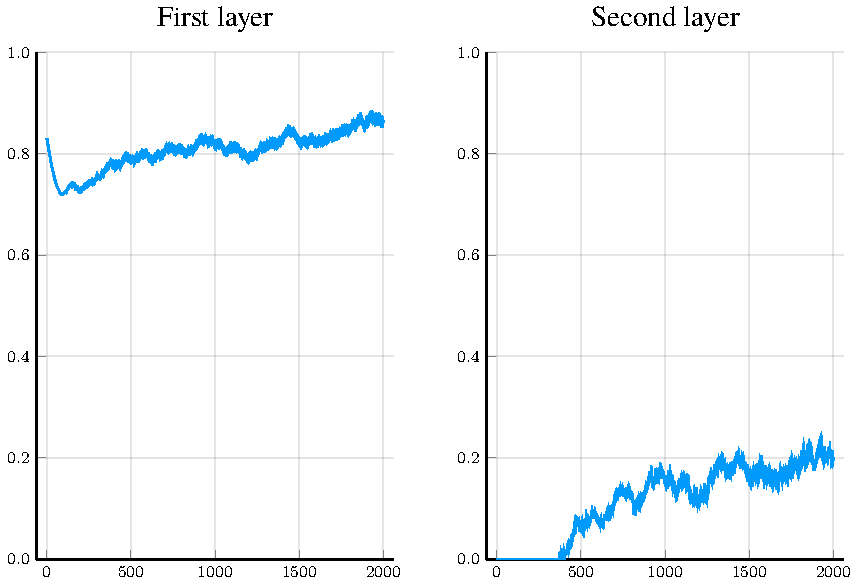
\includegraphics[width=\textwidth]{images/relu-difference-test/difference.pdf}
	\caption{Values of the test based on equation \ref{difference_test} over 2000 learning epochs}\label{difference_test_results}
\end{figure}

\begin{figure}
	\centering
	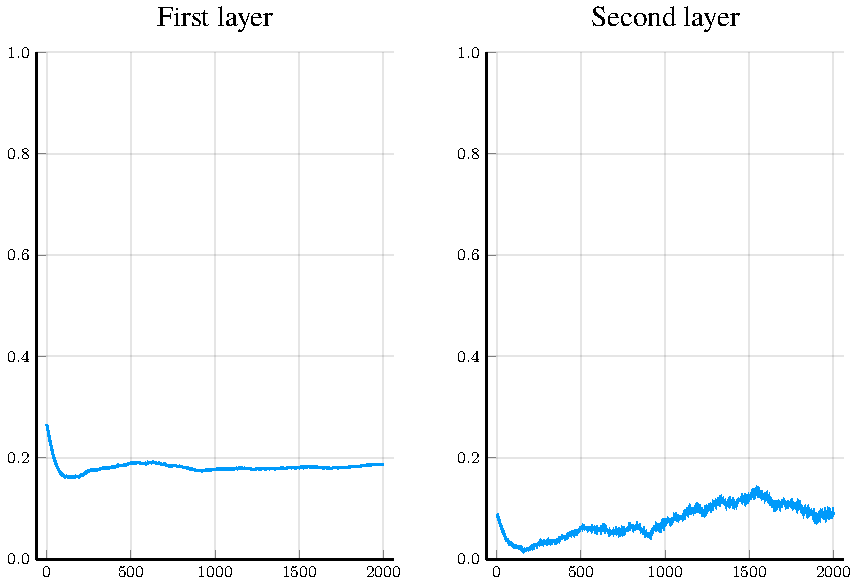
\includegraphics[width=\textwidth]{images/relu-average-test/average.pdf}
	\caption{Values of the test based on equation \ref{average_test} over 2000 learning epochs}\label{average_test_results}
\end{figure}

Based on the relatively hight values in both tests and on the fact that these values generally grow over the learning period, the tests don't support the outlined hypothesis. However, the tests alone don't present an evidence strong enough to reject the hypothesis -- e. g. the assertions made when designing these tests may not actually hold. \todo{Is it OK to say this?}

\section{Relation to theorem \ref{targetprop_works}}

An interesting metric which might provide some insight into the workings of target propagation is the angle between the actual target propagation update of the parameters and a theoretical update computed using the backpropagation algorithm. In theorem \ref{targetprop_works}, this angle is denoted \( \alpha \). Figure \ref{angle} shows the value of \( \alpha \) over the learning period. For the second layer, the angle is trivially 0 due to the choice of the last layer target using equation \ref{targetprop_last_layer_target}.

\begin{figure}
	\centering
	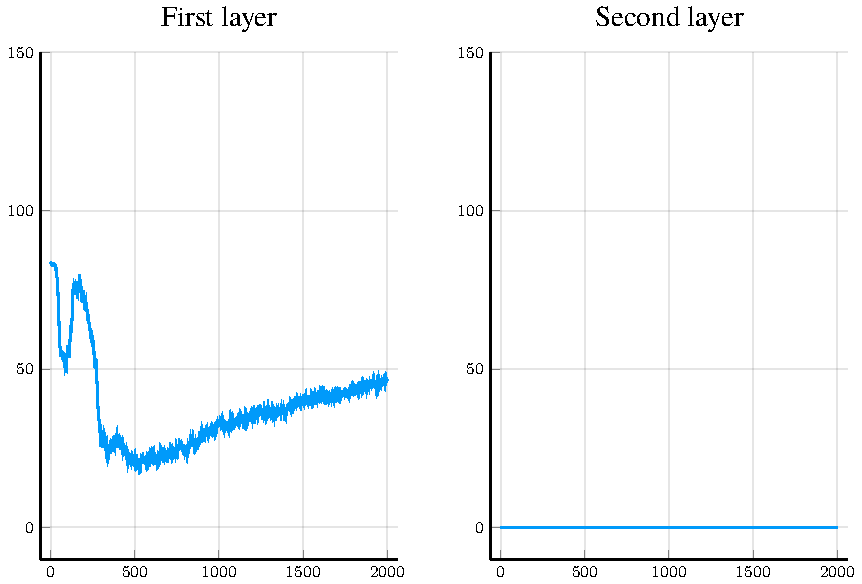
\includegraphics[width=\textwidth]{images/relu-angle/angle.pdf}
	\caption{Angle \( \alpha \) from theorem \ref{targetprop_works} (in degrees) over 2000 learning epochs}\label{angle}
\end{figure}

As can be seen in the figure, the angle between the backpropagation update and the targetpropagation update isn't close to 0 for the first layer. This phenomenon seems to contradict the claim of theorem \ref{targetprop_works}. In order to validate the implementation and to resolve this discrepancy, the lower bound on the cosine of the angle between \( \delta \VUmat{W}_{\mathrm{BP}}^{(i)} \) and \( \delta \VUmat{W}_{\mathrm{TP}}^{(i)} \) was computed for all the layers over the learning epochs. The terms \( \Delta_1 \left( \eta \right) \) and \(  \Delta_2 \left( \eta \right) \) were considered to be 0. Figure \ref{angle-bound} shows the development of the lower bound over the learning period. It is expressed as the upper bound on the angle, i. e. as the bound
\[ \cos^{-1} \left( \frac{\lambda_{\mathrm{min}}}{\lambda_{\mathrm{max}}} \right) > \alpha \]
Note that this upper bound considers the update of all parameters of the model, i. e. all the layers combined. Also note that due to the nature of the cosine function, the upper bound is invalid for angles over \( 90^\circ \).

\begin{figure}
	\centering
	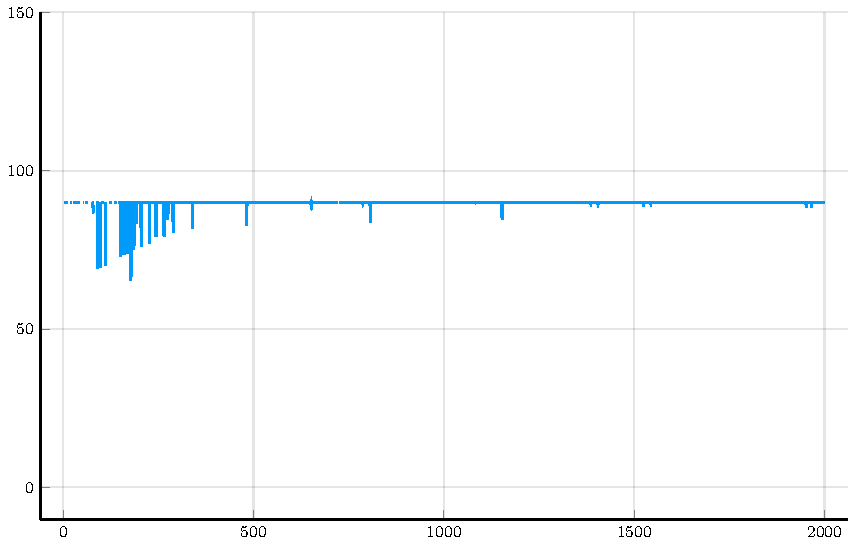
\includegraphics[width=\textwidth]{images/relu-angle-bound/angle-bound.pdf}
	\caption{Upper bound on the angle \( \alpha \) from theorem \ref{targetprop_works} (in degrees) over 2000 learning epochs}\label{angle-bound}
\end{figure}

When considered together with the actual angles, it is clear that the actual angles occasionally follow the general trend of the upper bound. For most of the learning period, the bound is very high however. That means that while the experiment satisfies theorem \ref{targetprop_works}, the theorem doesn't provide any actual limitation on the learning process and doesn't contradict the relative failure to learn.

\section{Learning using close approximations of the actual inverses}
The results of the previous section lead to the question of whether the model would learn using the actual inverses instead of the approximate inverse function \( \widetilde{f}^{(i)} \). As is asserted in section \ref{targetprop_general}, computing the actual inverse isn't always possible. It is, however, possible to use a stronger approximation for the inverse. The chosen approach was to use the Limited-memory Broyden-Fletcher-Goldfarb-Shanno algorithm (see \cite{liu_limited_1989}).

\todo{LBFGS results}

\todo{DTP}
